\documentclass{beamer}
\usepackage[utf8]{inputenc}
\usepackage{cite}
\usepackage{graphicx}
\usepackage{float}
\usepackage{fontawesome}
\usepackage{multicol}


% Beamer theme settings
\usetheme{CambridgeUS}
\usecolortheme{default}

\title{Collaborative System Coordination Design for Urban Crisis: Resolution Using Multi-Agent Technology}
\author{Team 05}
\date{\today}

\begin{document}

\begin{frame}
    \titlepage
\end{frame}

% Introduction
\section{Introduction}
\begin{frame}{Introduction}
    \begin{itemize}
        \item \textbf{Objective}: Design the cooperation and coordination mechanisms that will
        be used to solve the emergency response for fire-related emergencies in Lloret de Mar, Girona.
        \item \textbf{Teams Involved}:
            \begin{itemize}
                \item Emergency Services
                \item Firefighters
                \item Medical Services
                \item Public Communications
                \item \textit{Forensics}
            \end{itemize}
        \item \textbf{Overview}:
            \begin{itemize}
                \item For each crew: process definition and Pydantic outputs. 
                \item Agent interactions: flows and routers.
            \end{itemize}
    \end{itemize}
\end{frame}

\subsection{Emergency Services}
\begin{frame}{Emergency Services Process and Outputs}
        \begin{minipage}[b]{0.45\textwidth}
            \centering
            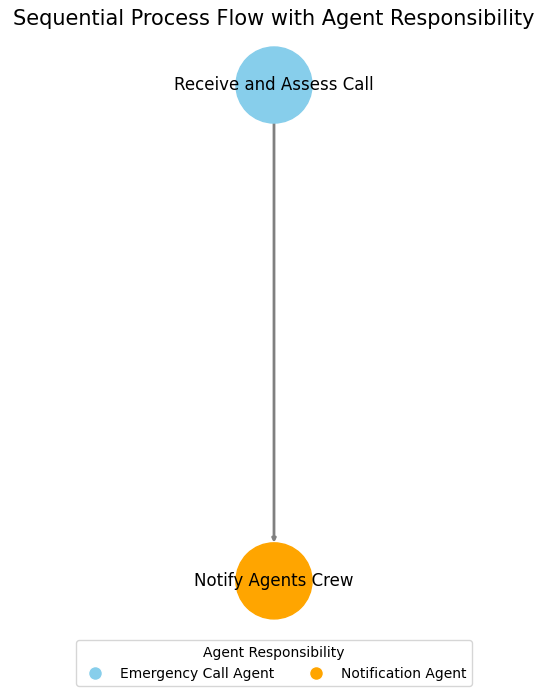
\includegraphics[width=0.75\linewidth]{figures/emergency_services_crew_flow.png}
        \end{minipage}
        \hfill
        \begin{minipage}[b]{0.5\textwidth}
            \begin{itemize}
                \item What type of fire is it?
                \item Where is it? 
                \item Is anyone injured? How badly? 
                \item How severe is the fire? 
                \item Are there hazards? 
                \item Is it an indoor or outdoor fire? 
                \item Is anyone inside or trapped? 
            \end{itemize}
            \vfill
        \end{minipage}
        \centering
            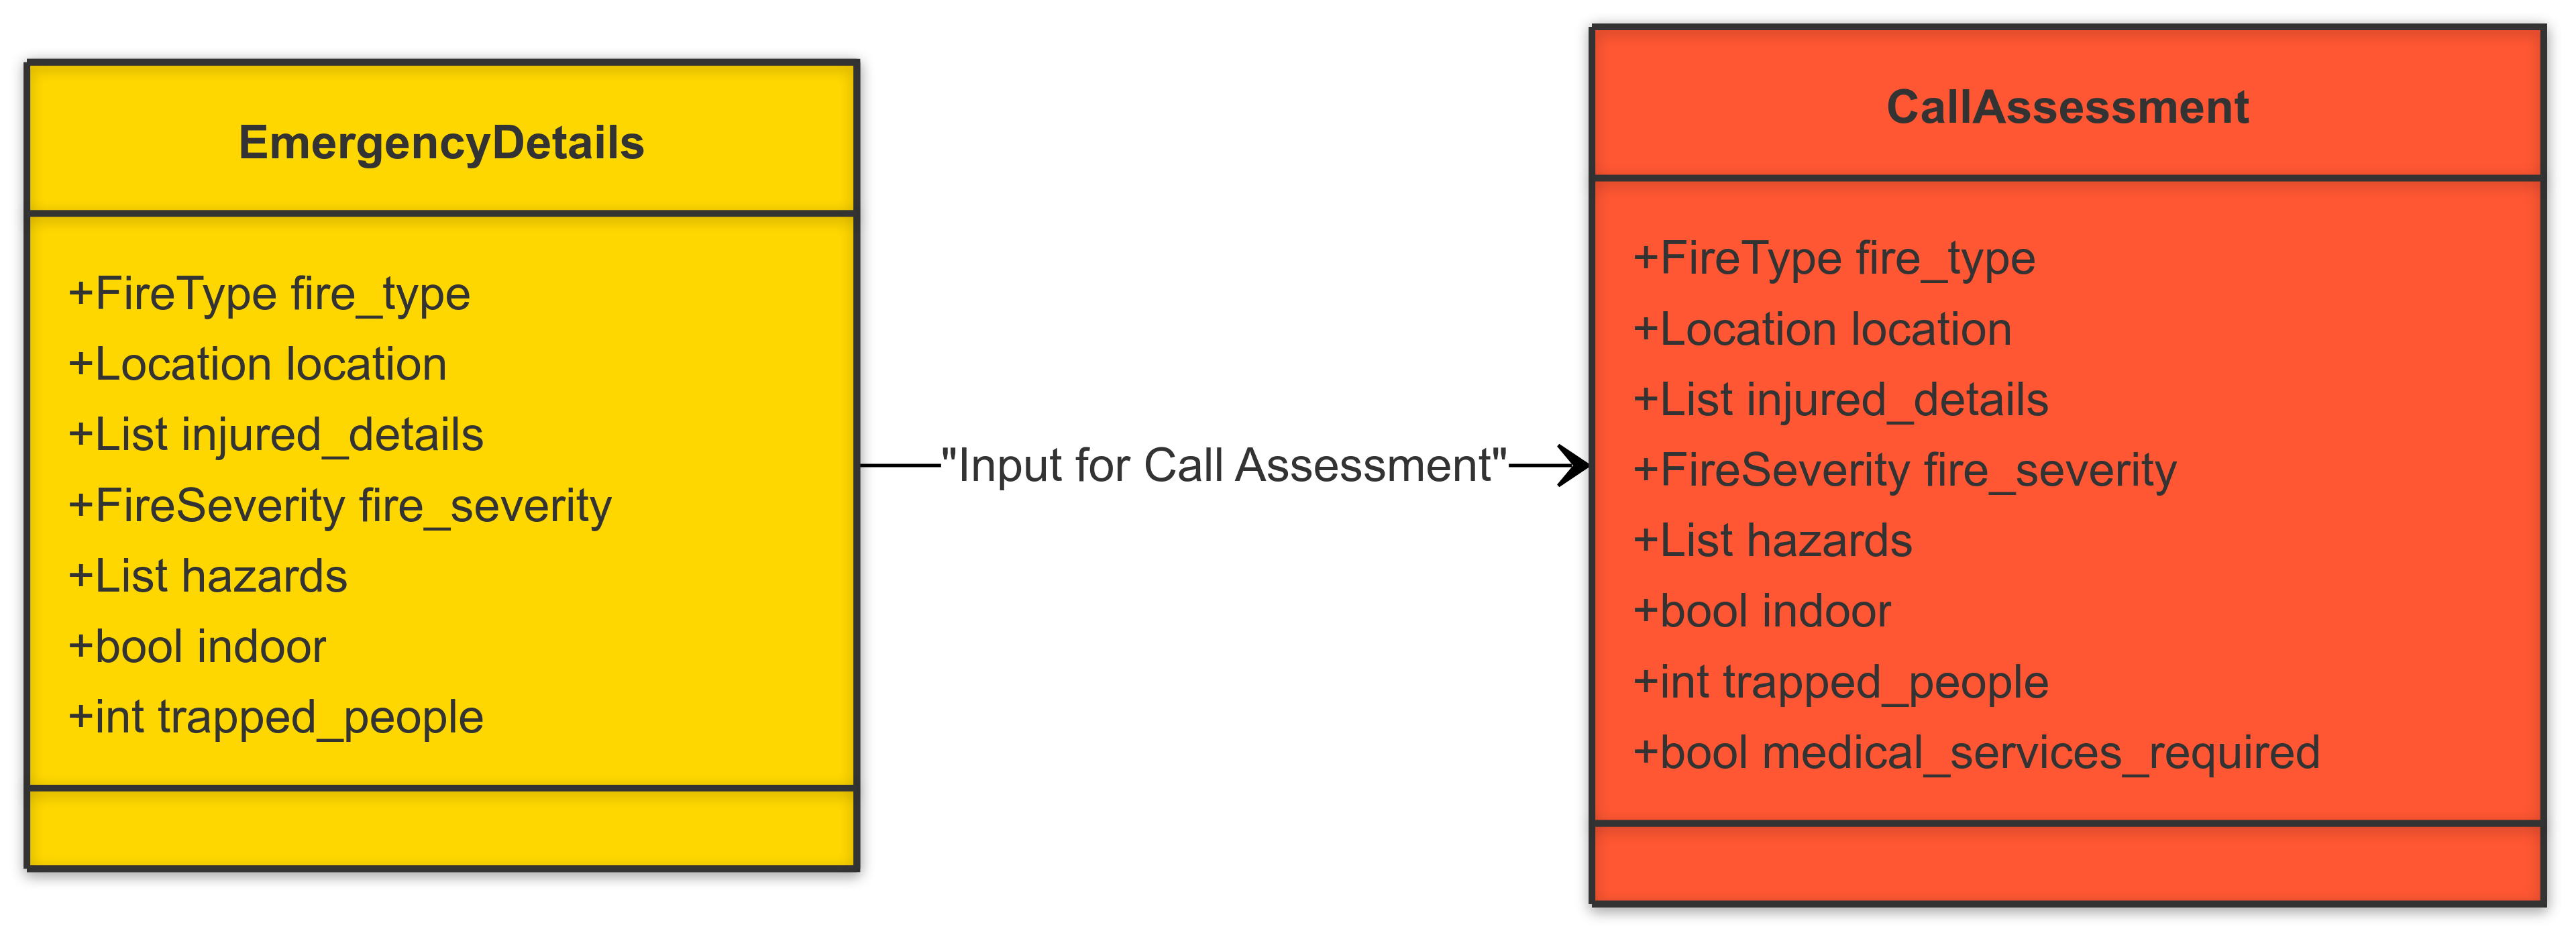
\includegraphics[width=0.7\linewidth]{figures/Emergency-Crew-Diagram.png}
\end{frame}



% Firefighters - Figure 1
\subsection{Firefighters}
\begin{frame}{Firefighters Process}
    \centering
    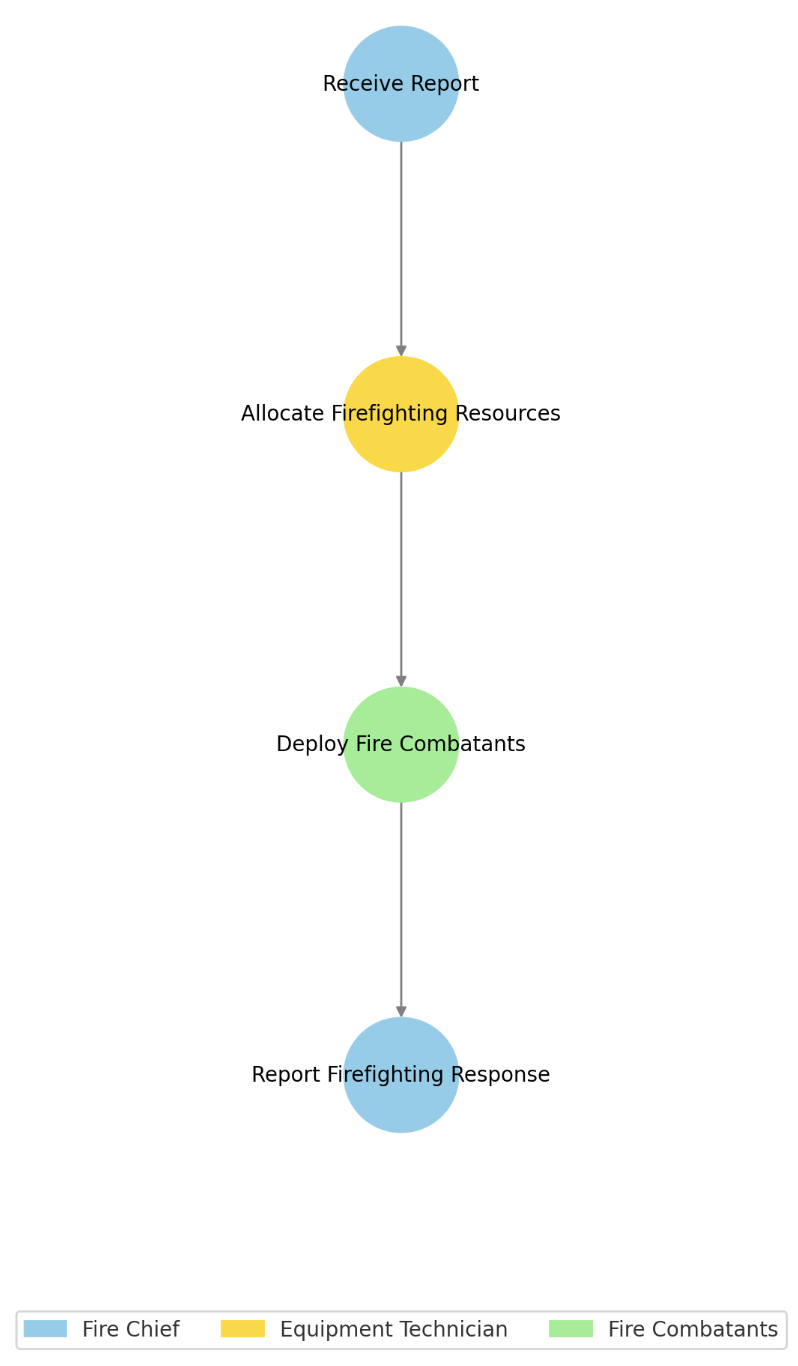
\includegraphics[height=\textheight]{figures/Firefighter_Crew_Flow.png}
\end{frame}

% Firefighters - Figure 2
\begin{frame}{Firefighters Outputs}
    \centering
    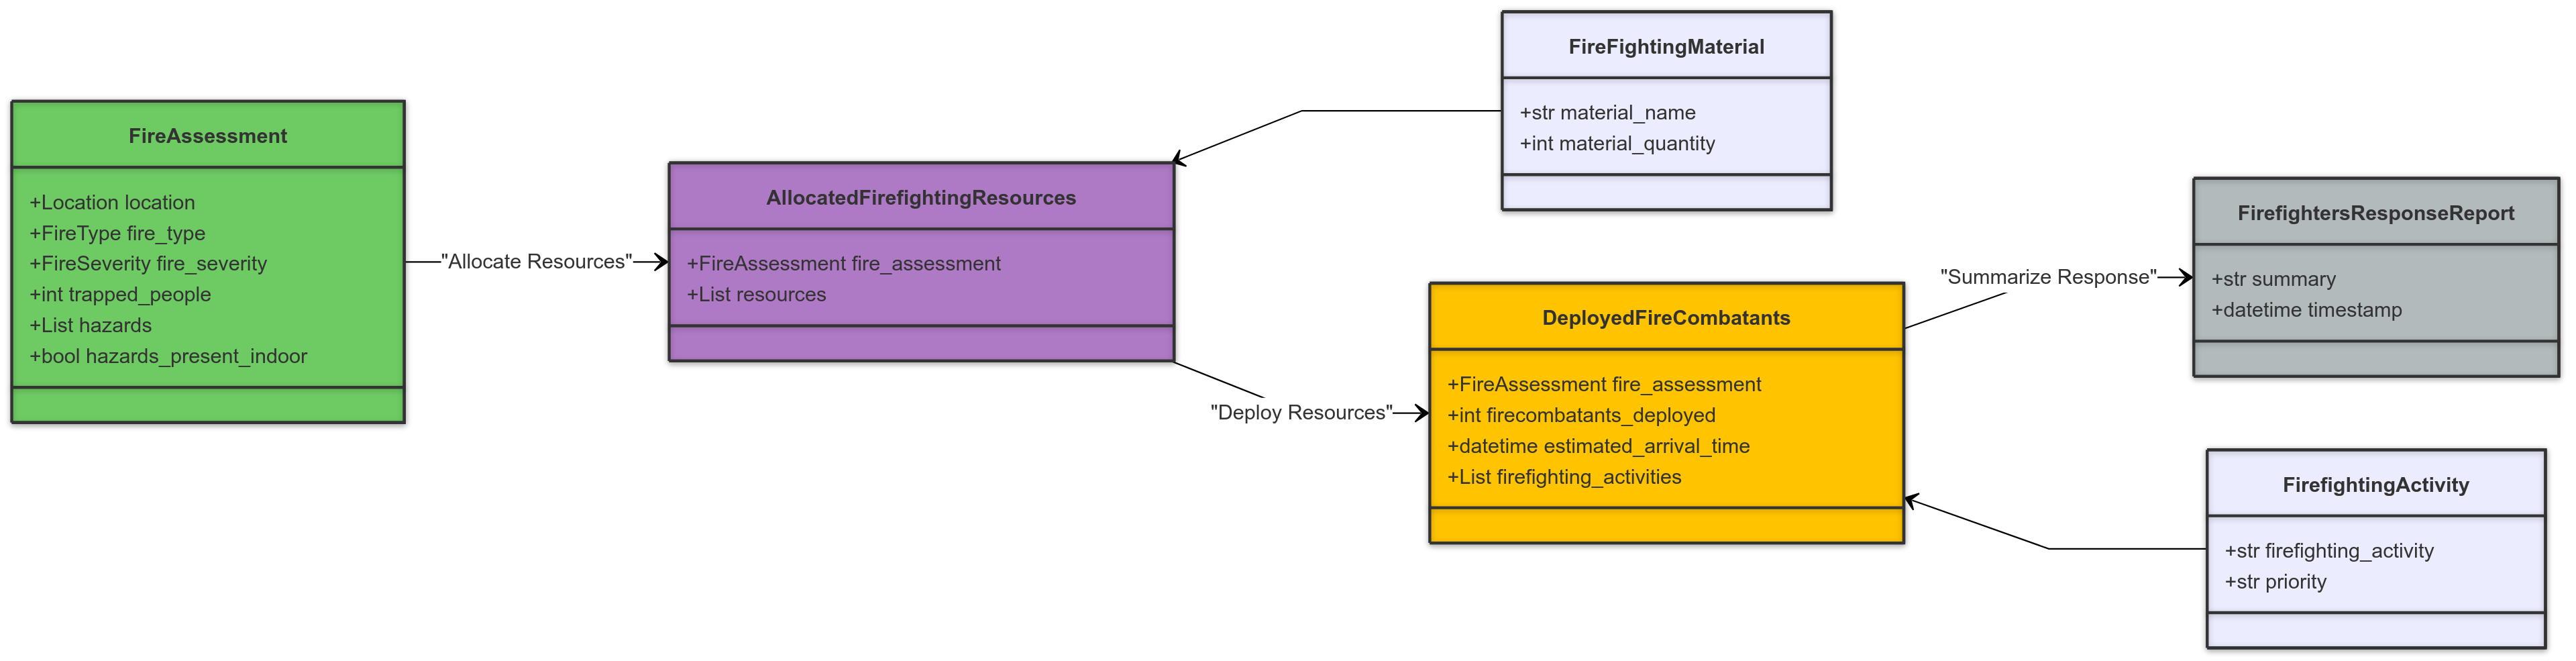
\includegraphics[width=\textwidth]{figures/Firefighters_ClassDiagram.png}
\end{frame}
% Medical Services - Figure 1
\begin{frame}{Medical Services Process}
    \centering
    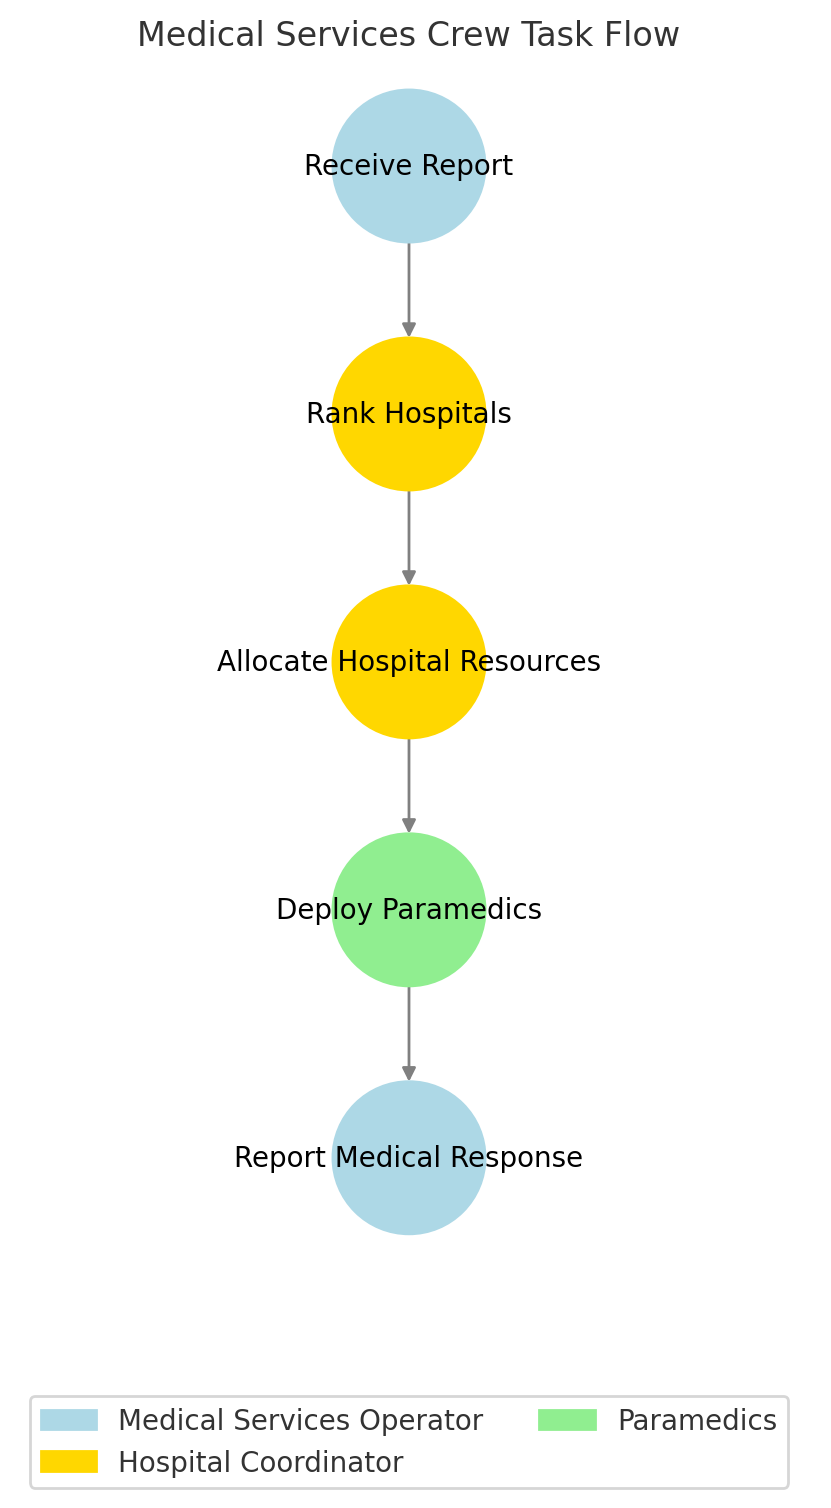
\includegraphics[height=\textheight]{figures/Medical_Services_Crew_Flow.png} 
\end{frame}

% Medical Services - Figure 2
\begin{frame}{Medical Services Outputs}
    \centering
    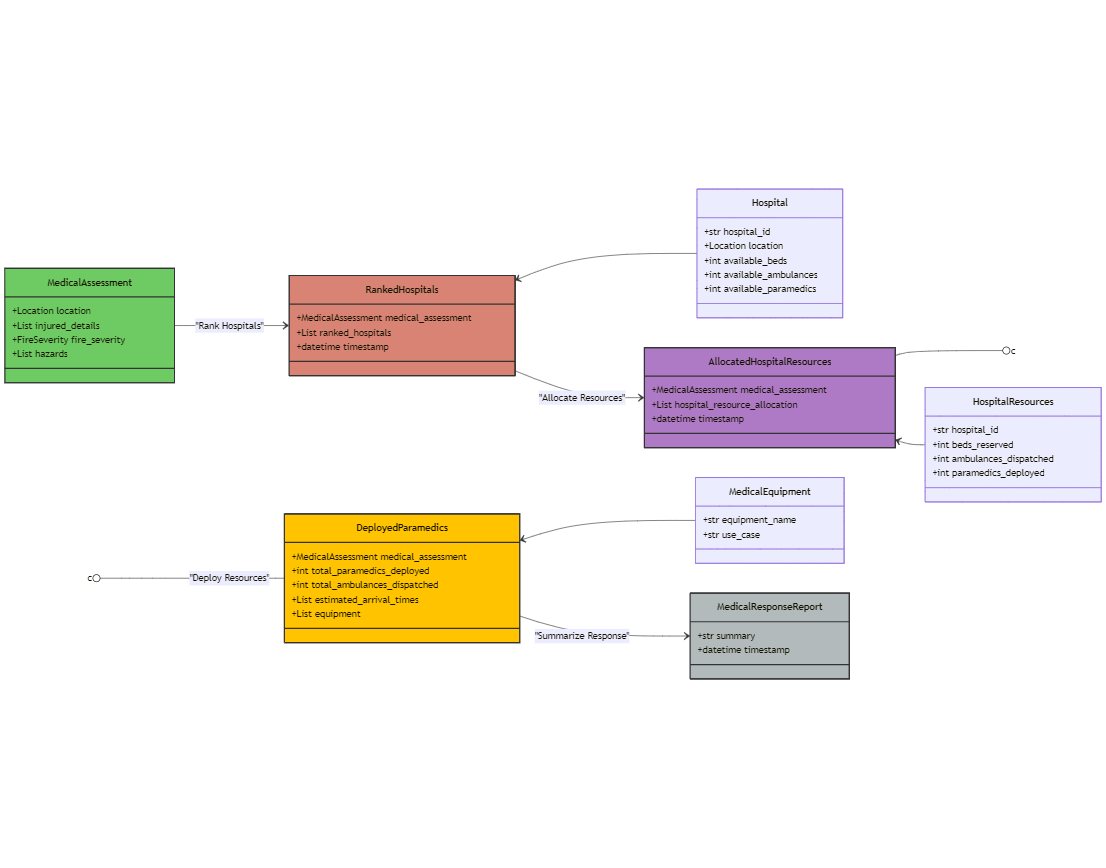
\includegraphics[width=\textwidth]{figures/MedicalServices_ClassDiagram.png}
\end{frame}
% Public Communications - Figure 1
\begin{frame}{Public Communications Process}
    \centering
    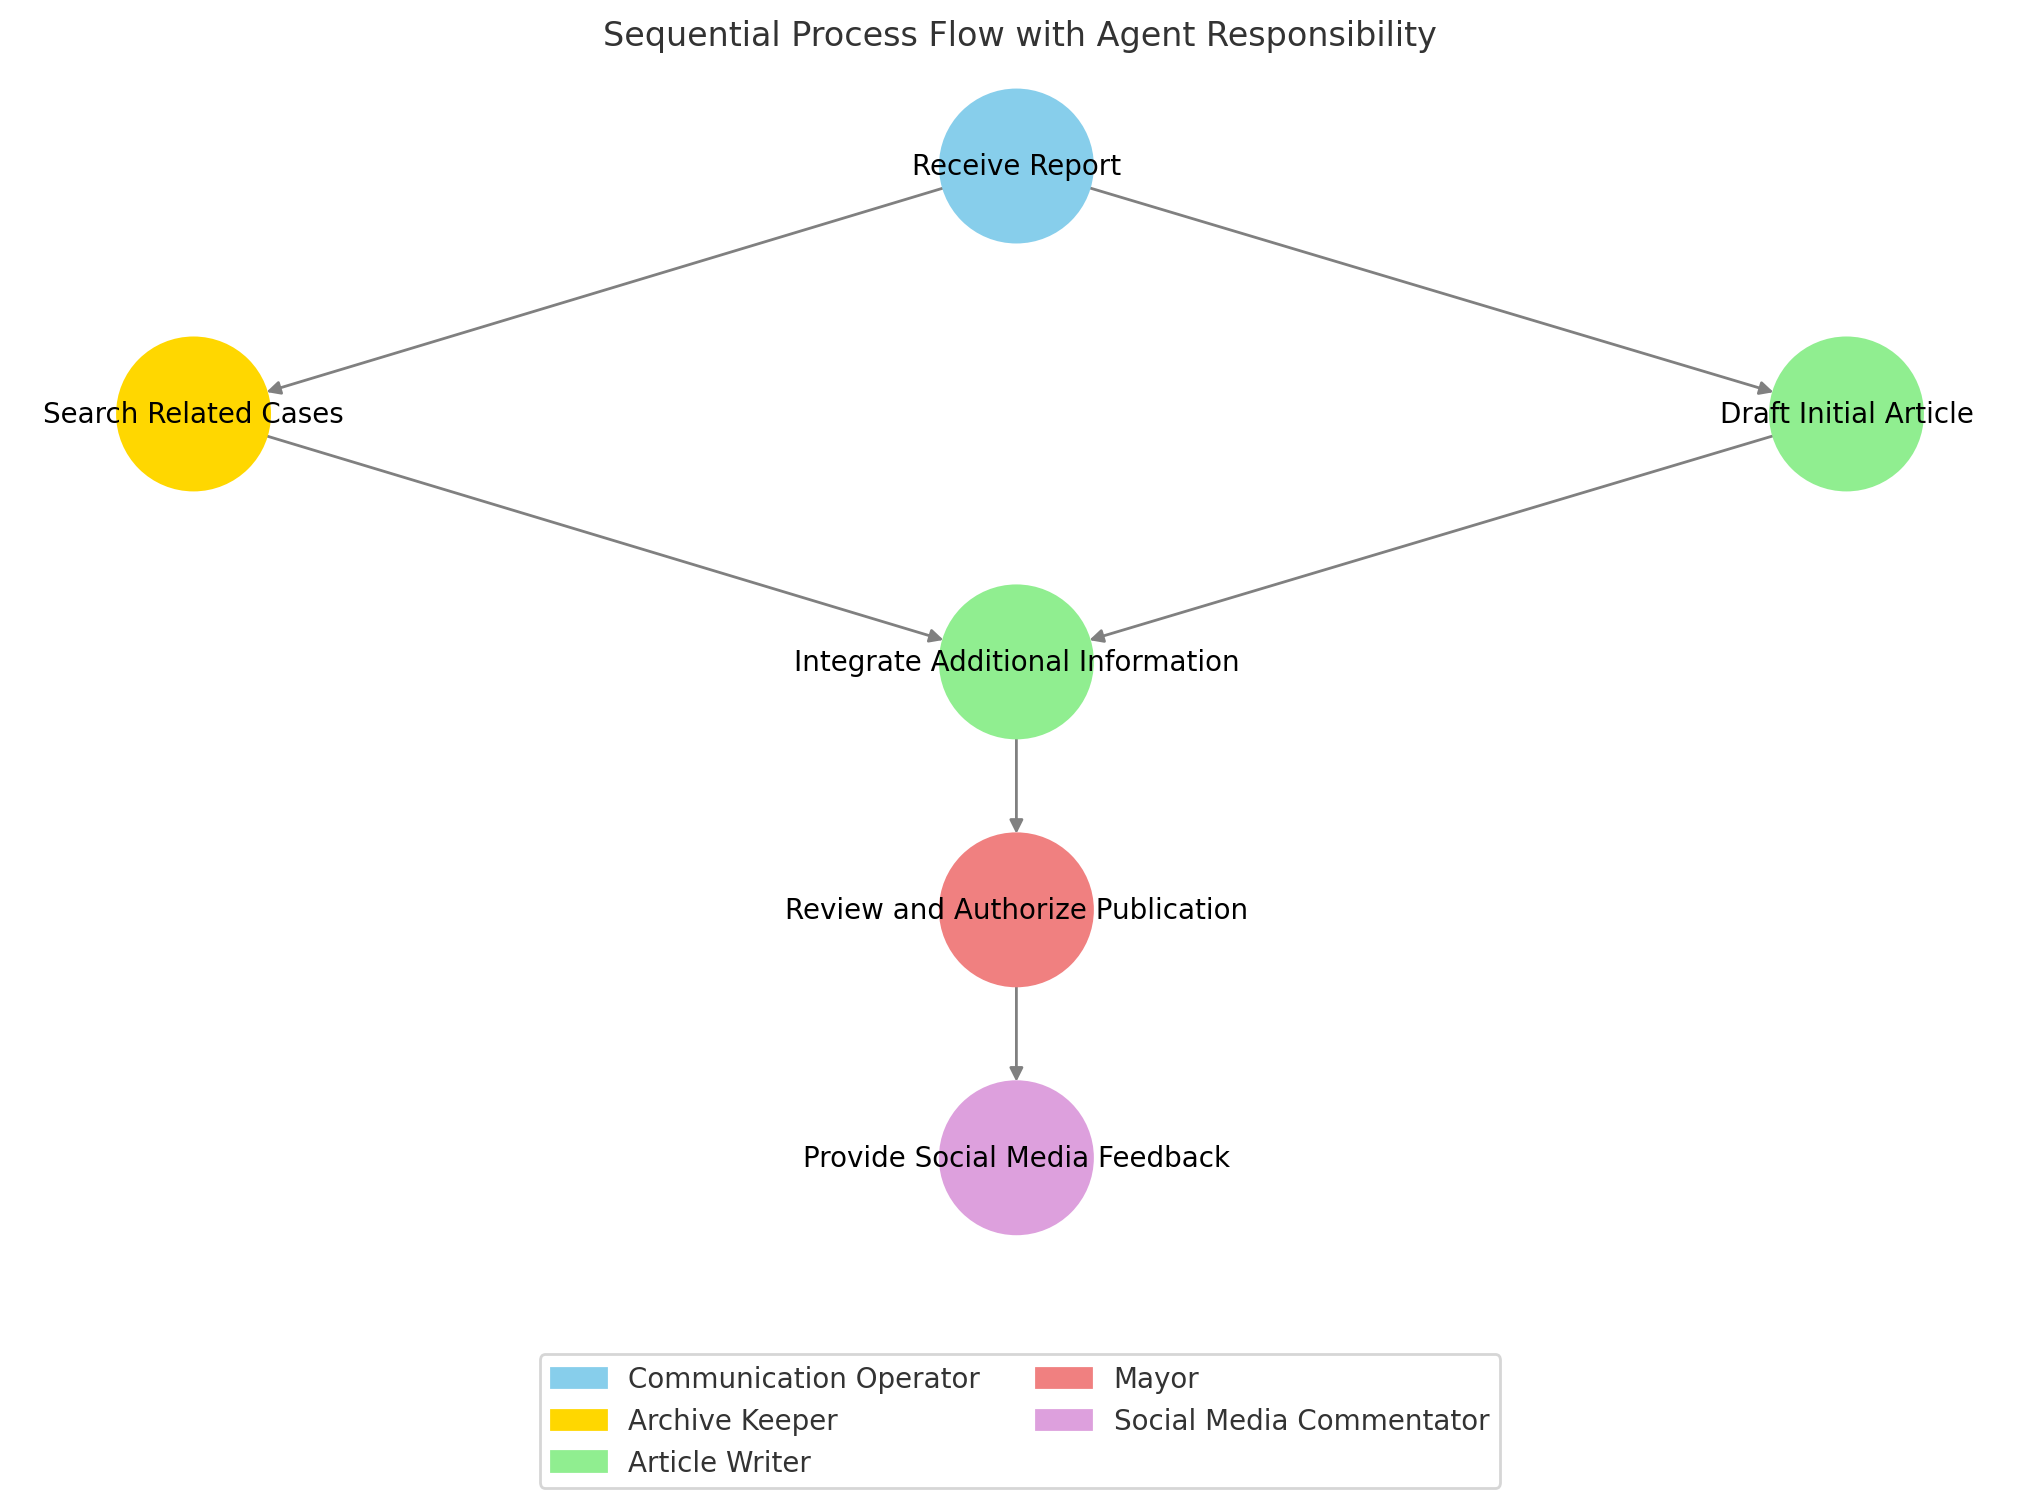
\includegraphics[width=\textwidth]{figures/PC-process.png} 
\end{frame}

% Public Communications - Figure 2
\begin{frame}{Public Communications Outputs}
    \centering
    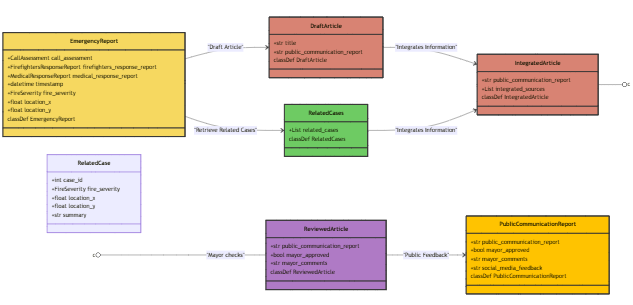
\includegraphics[width=\textwidth]{figures/PC-classDiagram.png}
\end{frame}

% References
\begin{frame}{References}
    \begin{itemize}
        \item Wooldridge, Michael. An Introduction to MultiAgent Systems. 2nd ed., John Wiley \& Sons, 2009. ISBN 978-0-470-51946-2.
        \item Wooldridge, Michael. "Properties of Intelligent Autonomous Agents." YouTube, 26 Feb. 2010, \url{https://www.youtube.com/watch?v=vID-_uIfAvg}.
    \end{itemize}
\end{frame}

\end{document}
